\documentclass[12pt,fleqn,answers]{exam}
%\usepackage{pifont}
%\usepackage{dingbat,bbding}

\usepackage{amssymb}
\usepackage[intlimits]{amsmath}
\usepackage{epsfig}
\usepackage{upgreek}
\usepackage[super]{nth}
\usepackage[colorlinks=true,linkcolor=black,anchorcolor=black,citecolor=black,filecolor=black,menucolor=black,runcolor=black,urlcolor=black]{hyperref}
\usepackage[letterpaper, margin=0.75in]{geometry}
\addpoints
\boxedpoints
\pointsinmargin
\pointname{pts}
\usepackage{tikz}
\usepackage{tkz-euclide}
\usetikzlibrary{shapes.geometric}
\usetikzlibrary{calc}
\usepackage[final]{microtype}
\frenchspacing
\usepackage[american]{babel}
\usepackage[T1]{fontenc}
\usepackage[]{fourier}
\usepackage{isomath}
\usepackage{upgreek,amsmath}
\usepackage{amssymb}
\usepackage{graphicx}

\newcommand{\dotprod}{\, {\scriptzcriptztyle\stackrel{\bullet}{{}}}\,}

\newcommand{\reals}{\mathbf{R}}
\newcommand{\lub}{\mathrm{lub}} 
\newcommand{\glb}{\mathrm{glb}} 
\newcommand{\complex}{\mathbf{C}}
\newcommand{\dom}{\mbox{dom}}
\newcommand{\range}{\mbox{range}}
\newcommand{\cover}{{\mathcal C}}
\newcommand{\integers}{\mathbf{Z}}
\newcommand{\vi}{\, \mathbf{i}}
\newcommand{\vj}{\, \mathbf{j}}
\newcommand{\vk}{\, \mathbf{k}}
\newcommand{\bi}{\, \mathbf{i}}
\newcommand{\bj}{\, \mathbf{j}}
\newcommand{\bk}{\, \mathbf{k}}
\DeclareMathOperator{\Arg}{\mathrm{Arg}}
\DeclareMathOperator{\Ln}{\mathrm{Ln}}
\newcommand{\imag}{\, \mathrm{i}}

\usepackage{graphicx}
\usepackage{color}
%\shadedsolutions
%\definecolor{SolutionColor}{rgb}{1,0.72,0.46} %{0.8,0.9,1}
\newcommand\AM{\textsc{am}}
\newcommand\PM{\textsc{pm}}
     
\newcommand{\quiz}{10}
\newcommand{\term}{Fall}
\newcommand{\due}{Tuesday 26 September 13:20}
\newcommand{\class}{MATH 202, Fall \the\year}
\begin{document}
\large
\vspace{0.1in}
\noindent\makebox[3.0truein][l]{\textbf{\class}}
\textbf{Name:} \hrulefill \\
\noindent \makebox[3.0truein][l]{\textbf{In class work  \quiz}}
\textbf{Row and Seat}:\hrulefill\\
\vspace{0.1in}
\small
\vspace{0.1in}
\noindent  In class work  \textbf{\quiz\/}  has questions \textbf{1} through  \textbf{\numquestions} \/ with a total of \textbf{\numpoints\/}  points.   
Turn in your work at the end of class  \emph{on paper}. This assignment is due \emph{\due}.

\vspace{0.1in}

Here are some results that you might like to use
\begin{align*}
 {{\cos{(x)}}^{2}} &=\frac{\cos{\left( 2 x\right) }}{2}+\frac{1}{2},\\
 {{\cos{(x)}}^{4}} &=\frac{\cos{\left( 4 x\right) }}{8}+\frac{\cos{\left( 2 x\right) }}{2}+\frac{3}{8}, \\
 {{\sin{(x)}}^{2}} &=\frac{1}{2}-\frac{\cos{\left( 2 x\right) }}{2}, \\
 {{\cos{(x)}}^{2}}\, {{\sin{(x)}}^{2}}&=\frac{1}{8}-\frac{\cos{\left( 4 x\right) }}{8},\\
 {{\cos{(x)}}^{4}}\, {{\sin{(x)}}^{2}} &=-\frac{\cos{\left( 6 x\right) }}{32}-\frac{\cos{\left( 4 x\right) }}{16}+\frac{\cos{\left( 2 x\right) }}{32}+\frac{1}{16},\\ 
 {{\sin{(x)}}^{4}}&=\frac{\cos{\left( 4 x\right) }}{8}-\frac{\cos{\left( 2 x\right) }}{2}+\frac{3}{8}, \\ 
 {{\cos{(x)}}^{2}}\, {{\sin{(x)}}^{4}} &=\frac{\cos{\left( 6 x\right) }}{32}-\frac{\cos{\left( 4 x\right) }}{16}-\frac{\cos{\left( 2 x\right) }}{32}+\frac{1}{16}, \\
 {{\cos{(x)}}^{4}}\, {{\sin{(x)}}^{4}} &=\frac{\cos{\left( 8 x\right) }}{128}-\frac{\cos{\left( 4 x\right) }}{32}+\frac{3}{128}.
\end{align*}
\begin{questions}

    \question[2]  Use Desmos to sketch the region $Q$ defined as $Q = \{(x,y) \mid 0 \leq y \leq x^4 \sqrt{1-x^2}
    \mbox{ and } 0 \leq x \leq 1 \}$. Duplicate
    the graph here.
    \begin{solution}[2.0in]
      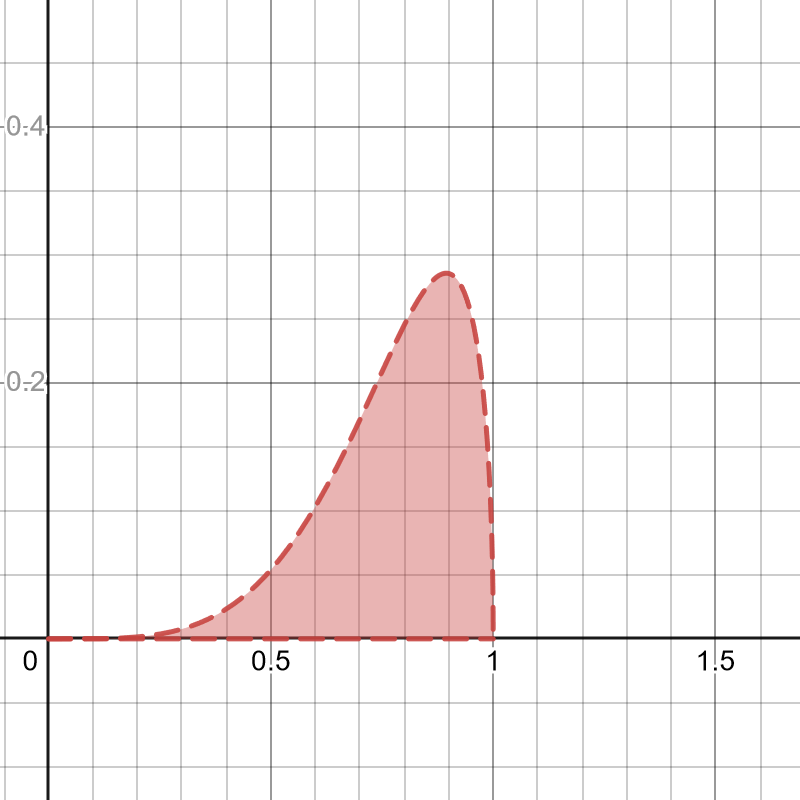
\includegraphics[scale=0.2]{desmos-graph(60).png}
    \end{solution}
    
    \question[2] Find $\mbox{area}(Q)$.
  \begin{solution}%[2.0in]
    We need to find $\text{Area}(Q) = \int_0^1 x^4 \sqrt{1-x^2} \, \mathrm{d} x$.
    Let $x = \sin(\theta)$. Then when $x = 0$, we have $\theta=0$;
    and $x = 1$, implies $\theta = \uppi/2$. So
    We have
    \begin{align*}
    \int_0^1 x^4 \sqrt{1-x^2} \, \mathrm{d} x &= \int_0^{\uppi/2} \sin(x)^4 \cos(x)^2 \, \mathrm{d} x, \\
                &= \int_0^{\uppi/2}  \frac{\cos{\left( 6  \, \theta \right) }}{32}-\frac{\cos{\left( 4   \,\theta \right) }}{16}-\frac{\cos{\left( 2  \, \theta \right) }}{32}+\frac{1}{16} \, \mathrm{d} \theta \\
                &= \left. \frac{\sin{\left( 6 \, \theta \right) }}{192}-\frac{\sin{\left( 4   \,\theta \right) }}{64}-\frac{\sin{\left( 2 \theta \right) }}{64}+\frac{\theta }{16} \right |_0^{\uppi/2}, \\
                &= \frac{\uppi}{32}.
  \end{align*}
    \end{solution}
      %  \newpage
        \question[2] Using your graph, make a pretty good guess for the x-coordinate to the centroid of $Q$.
  \begin{solution}[1.0in]
    I think the x coordinate of the center of the centroid is close to 
    the relative maximum of the function; so I'm going to guess that
    $\overline{x} \approx \frac{9}{10}$
   
    \end{solution}
    

    
       \question[2] Find the x-coordinate to the centroid of $Q$.
  \begin{solution}[2.0in] 
    We need to evaluate $\int_0^1 x^5 \sqrt{1-x^2} \, \mathrm{d} x$.
    The MATH 115 way to do this is to substitute $z = 1-x^2$. That 
    works OK.  The MATH 202 way is to substitute $x = \sin(\theta)$.
    Let's try the MATH 202 way:
    \begin{align*}
     \int x^5 \sqrt{1-x^2} \, \mathrm{d}x &= 
     \int \sin(\theta)^5 \cos(\theta)^2  \, \mathrm{d}\theta\\
     &= \int \sin(\theta) (1- \cos(\theta)^2)^2 \cos(\theta)^2  \, \mathrm{d}\theta\\
     &= -\int (1-z^2)^2 z^2 \, \mathrm{d} z,\\
     &= -\int z^2 - 2 z^4  + z^6 \, \mathrm{d} z,\\
     &= -\frac{1}{3} z^3 +\frac{2}{5} z^5 - \frac{1}{7} z^7, \\
     &= -\frac{1}{3} \cos(\theta)^3 +\frac{2}{5} \cos(\theta)^5 - \frac{1}{7} \cos(\theta)^7,\\
     &= -\frac{1}{3}\cos(\arcsin(x))^3 + \frac{2}{5} \cos(\arcsin(x))^5 - \frac{1}{7} \cos(\arcsin(x))^7,\\
          \end{align*}
   So for the definite integral, we have
   \begin{equation}
    \int_0^1  x^5 \sqrt{1-x^2} \, \mathrm{d}x
     = \left(0 + 0 + 0 \right) - \left(-\frac{1}{3} + \frac{2}{5} - \frac{1}{7}\right)
     = \frac{8}{105}
   \end{equation}   
   So $\text{Area}(Q) \overline{x} = \frac{8}{105}$, so
   $\overline{x} = \frac{8}{105} \times \frac{32}{\uppi}
   = \frac{256}{105 \uppi} \approx 0.7760698177433374.$
    \end{solution}
\end{questions}

\end{document}

